%-----------------------------------
%-----------------------------------
% Msc Dissertation / Phd Thesis Template - Minds Lab
% Based on Abntex2
% Updated: November, 2018
%-----------------------------------
%-----------------------------------

\documentclass[
	12pt,				
	openright,			
	twoside,			
	a4paper,
	%brazil, % Texts in pt-br
	english			
]{abntex2}

%-----------------------------------
% Basic packages
%-----------------------------------
\usepackage[T1]{fontenc}		% Font
%\usepackage{times}
\usepackage[utf8]{inputenc}		% Special pt-br characters
\usepackage{lastpage}			% Catalographic card
\usepackage{indentfirst}		% Indent 1st paragraph
\usepackage{color}				
\usepackage{graphicx}			
\usepackage{microtype} 			% Justify (left and right side) 
\usepackage{makeidx}            % Remissive Index
\usepackage{pdfpages}           % Add pdf pages

%-----------------------------------
% Additional packages
%-----------------------------------
\usepackage{amsmath,amsfonts,amssymb}
\usepackage[table]{xcolor}
\usepackage{multirow}           % Merge rows and columns in tables
\usepackage{longtable}          % Large tables
\usepackage{fancyvrb}           % Codes and Outputs commands
\usepackage{listings}           % Codes and Outputs commands
\usepackage{pdflscape}
\usepackage{float}
\usepackage[authoryear]{natbib} % Authors imputation
\usepackage{subfig}             % Subfigures
\usepackage{latexsym}           % Extra symbols of Latex
\usepackage{booktabs}
\usepackage{enumerate}
\usepackage{acronym}
\usepackage{algorithm}          % Algorithms
%\usepackage[portuguese, ruled, linesnumbered]{algorithm2e} %to portuguese text, include this linha and comment the top row: \usepackage{algorithm}  
\usepackage[noend]{algpseudocode}
\usepackage{url}
\let\realurl\url
\renewcommand{\url}[1]{\realurl{#1}\wlog{URLX #1}}
\usepackage{lipsum}				% To generate dummy text

%-----------------------------------
% Box the algorithm
\makeatletter
\def\BState{\State\hskip-\ALG@thistlm}
\makeatother

%-----------------------------------
% Front pages
%-----------------------------------
\titulo{Template for Dissertations and Thesis}
\autor{Emma Thomas}
\local{Belo Horizonte}
\data{2018}
\orientador{Advisor: Rita Levi-Montalcini}
\coorientador{Co-advisor: Nikola Tesla}
\instituicao{%
 	FEDERAL UNIVERSITY OF MINAS GERAIS \\
 	School of Engineering \\
 	Graduate Program in Electrical Engineering
 	\newline
 	\newline
}

\tipotrabalho{Thesis (Doctorate)}
%\preambulo{Tese de Doutorado submetida à Banca	Examinadora 
% designada pelo Colegiado do Programa de Pós-Graduação em Engenharia Elétrica
% da Escola de Engenharia da Universidade Federal de Minas Gerais, como
% requisito para obtenção do Título de Doutor em Engenharia Elétrica.} 
\preambulo{Final thesis presented to the Graduate Program in Electrical Engineering  of  the  Federal  University  of  Minas  Gerais  in
partial  fulfillment  of  the  requirements  for  the  degree  of Doctor in Electrical Engineering.}

%-----------------------------------
% Set the final PDF
%-----------------------------------
\definecolor{blue}{RGB}{41,5,195} % setting the blue color

% PDF informations
\makeatletter                   
\hypersetup{
     	%pagebackref=true,
		pdftitle={\@title}, 
		pdfauthor={\@author},
    	pdfsubject={\imprimirpreambulo},
	    pdfcreator={LaTeX with abnTeX2},
		pdfkeywords={abnt}{latex}{abntex}{abntex2}{trabalho acadêmico}, 
		colorlinks=true,        % false: boxed links; true: colored links
    	linkcolor=blue,         % color of internal links
    	citecolor=blue,        	% color of links to bibliography
    	filecolor=magenta,      % color of file links
		urlcolor=blue,
		bookmarksdepth=4
}
\makeatother

%-----------------------------------
% Spacing between lines and paragraphs
%-----------------------------------
\setlength{\parindent}{1.5cm}   % Set length of indent
\setlength{\parskip}{0.2cm}     % Set length among the paragraphs 

%Index
\makeindex


% Muda a numeração de página (de todas as páginas) para o canto superior direito.
% Comentando este bloco de código vai fazer com que seja impresso tipo livro.
\makepagestyle{abntheadings}
\makeevenhead{abntheadings}{\ABNTEXfontereduzida\textit\rightmark}{}{\ABNTEXfontereduzida\thepage}
\makeoddhead{abntheadings}{\ABNTEXfontereduzida\textit\rightmark}{}{\ABNTEXfontereduzida\thepage}
\makeheadrule{abntheadings}{\textwidth}{\normalrulethickness}


%-----------------------------------
% Main document
%-----------------------------------
\begin{document}

%-----------------------------------
%Language
%\selectlanguage{brazil}        % Texts in pt-br
\selectlanguage{english} 
\frenchspacing                  % Remove obsolete spaces between phrases

%-----------------------------------
% Pre-textual elements
\pretextual

%-----------------------------------
% Cover
\imprimircapa                   

% Folha de rosto
\imprimirfolhaderosto* % (o * indica que haverá a ficha bibliográfica)


%-----------------------------------
% Cataloguing data

% Manually
% \begin{fichacatalografica}
%     \includepdf{fig_ficha_catalografica.pdf}
% \end{fichacatalografica}

% or
% Automatically
\begin{fichacatalografica}
    \rmfamily
	%\sffamily
	\vspace*{\fill}					
	\begin{center}					
	\fbox{
    	\begin{minipage}[c][8cm]{13.5cm}		% Largura
        	\small
        	\imprimirautor              %Sobrenome, Nome do autor
        	\hspace{0.5cm} \imprimirtitulo  / \imprimirautor. --
        	\imprimirlocal, \imprimirdata-
        	\hspace{0.5cm} \pageref{LastPage} p. : il. (algumas color.) ; 30 cm.\\
        	\hspace{0.5cm} \imprimirorientadorRotulo~\imprimirorientador\\
        	\hspace{0.5cm}
        	\parbox[t]{\textwidth}{\imprimirtipotrabalho~--~\imprimirinstituicao,
        	\imprimirdata.}\\
        	\hspace{0.5cm}
            	1. Palavra-chave1.
        		2. Palavra-chave2.
        		2. Palavra-chave3.
        		I. Orientador.
        		II. Universidade Federal de Minas Gerais.
        		III. Escola de Engenharia.
        		IV. Título. 			
    	\end{minipage}
	}
	\end{center}
\end{fichacatalografica}

\newpage

%-----------------------------------
% Dedication 
\begin{dedicatoria}
   \vspace*{\fill}
   \centering
   \noindent
   \textit{Dedication here...} 
   \vspace*{\fill}
\end{dedicatoria}

%-----------------------------------
% Acknowledgments
\begin{agradecimentos}
Acknowledgments...

\end{agradecimentos}

%-----------------------------------
% Epigraph
\begin{epigrafe}
    \vspace*{\fill}
	\begin{flushright}
		\textit{Epigraph...}
	\end{flushright}
\end{epigrafe}

%-----------------------------------
% Resumo (abstract in Portuguese)
\setlength{\absparsep}{18pt} % set spacing between the paragraphs

\begin{resumo}
    O resumo deve ser feito em português. O resumo é elemento obrigatório e consiste em um texto conciso que representa os pontos relevantes do texto, devendo conter de 150 a 500 palavras. Ele deve abarcar o objeto da pesquisa, os objetivos, a metodologia, os resultados e a conclusão. Um abstract é um breve resumo de um artigo de pesquisa, tese, revisão, conferência, proceeding ou qualquer análise aprofundada sobre um determinado assunto ou disciplina, e é frequentemente usado para ajudar o leitor a tomar conhecimento rapidamente do propósito do texto. Ele é a versão precisa, sintetizada e seletiva do seu documento, dando destaque aos elementos mais importantes. O resumo também possui uma estrutura própria, deve dar uma breve introdução ao seu tema, evidenciar os objetivos, métodos empregados, resultados e conclusões, permitindo ao leitor vislumbrar todo o conteúdo da sua dissertação ou tese. Não é regra, mas é sugerido que ele seja escrito em um parágrafo único, direto, e possivelmente caber em uma página. 
    
        
    Palavras-chave: Palavra-chave1. Palavra-chave2. Palavra-chave3. Palavra-chave4. Palavra-chave5.

\end{resumo}

%-----------------------------------
% Abstract (in English)
\begin{resumo}[Abstract]
    \begin{otherlanguage*}{english}
        An abstract is a self-contained, short, and powerful statement that describes a larger work. Components vary according to discipline. An abstract of a social science or scientific work may contain the scope, purpose, results, and contents of the work. An abstract of a humanities work may contain the thesis, background, and conclusion of the larger work. An abstract is not a review, nor does it evaluate the work being abstracted. While it contains key words found in the larger work, the abstract is an original document rather than an excerpted passage.
        
        \url{https://users.ece.cmu.edu/~koopman/essays/abstract.html}

        \textit{Keywords: Keyword 1.. Keyword 2. Keyword 3. Keyword 4. Keyword 5.}
    \end{otherlanguage*}
\end{resumo}

%-----------------------------------
% Figures list
\pdfbookmark[0]{\listfigurename}{lof}
\listoffigures*
\cleardoublepage

%-----------------------------------
% Tables list
\pdfbookmark[0]{\listtablename}{lot}
\listoftables*
\cleardoublepage

%-----------------------------------
% Algorithms list
\pdfbookmark[0]{\listtablename}{loa}
\listofalgorithms
\cleardoublepage

%-----------------------------------
% Abbreviations
%-----------------------------------
% Abbreviations and acronyms
%-----------------------------------

\begin{siglas}
  \item[ABNT] Associação Brasileira de Normas Técnicas
  \item[MINDS] Machine Intelligence and Data Science
  \item[UFMG] Universidade Federal de Minas Gerais
  \item[SVM] Support Vector Machine
\end{siglas}
\cleardoublepage

%-----------------------------------
% Symbols
%-----------------------------------
% Symbols
%-----------------------------------

\begin{simbolos}
  \item[$ \Gamma $] Gama
  \item[$ \Lambda $] Lambda
  \item[$ \zeta $] zeta
  \item[$ \alpha $] alpha
\end{simbolos}
\cleardoublepage

%-----------------------------------
% Summary
\pdfbookmark[0]{\contentsname}{toc}
\tableofcontents*
\cleardoublepage


%-----------------------------------
% TEXTUAL ELEMENTS
%-----------------------------------
\textual

%-----------------------------------
% Chapters
\chapter[Introduction]{Introduction} 
\label{chp1_introduction} %label means how to call these title in your text in the future 

The aim of this document is to present a basic template for elaboration of dissertations and thesis using \LaTeX 
and \textbf{abntex2} class, Standard \texttt{ABNT NBR 10520: 2002}. 

The chapter \texttt{Introduction} presents, basically, the concepts within a \texttt{Context}, identifies the \texttt{Problem} and presents the \texttt{Solution}. Lastly, but not least, you can submit further details as well as give search leads.

Bla bla bla ....

The rest of the document is organized as follows: Chapter \ref{chp2_elements} presents the main elements, such as references, figures, tables, equations, algorithms and other explanatory elements. Chapter \ref{chp3_methodology} presents random dummy text. Chapter \ref{chp4_results} presents random dummy text. Chapter \ref{chp5_conclusion} presents some comments and final observations. Lastly, see either an example of Appendix \ref{apendiceA} or Annex \ref{anexoA}.




\chapter[Elements]{Elements} 
\label{chp2_elements} 

This chapter presents examples of how to cite some references, how to use figures, tables, equations, algorithms and other explanatory elements.

%-----------------------------------
\section{Citations}

The Standard \texttt{ABNT NBR 10520: 2002} describes that \index{quotations} short direct quotations with (less than three lines) must be described with ``double quotes'' around it. Otherwise, \index{direct quotations}long direct quotations (up to three lines) must be highlighted with a 4cm indentation of the left margin, with lower than the used text and without the quotation marks. To do this, use the citation environment, as the example:

\begin{citacao}
For example, if the probability of an event is not known with precision, then it may be characterized linguistically as, say, quite likely, not very unlikely, highly unlikely, etc., where quite likely, not very unlikely and highly unlikely are interpreted as labels of fuzzy subsets of the unit interval. Such subsets may be likened to ball-parks without sharply defined boundaries which serve to provide an approximate rather than exact characterization of the value of a variable \citep{zadeh1976fuzzy}.
\end{citacao}

%-----------------------------------
\section{References}

Throughout your dissertation or thesis, you can use the references in two main ways: 1) automatically link from bibliographic management softwares Mendeley\footnote{www.mendeley.com}, Zotero\footnote{www.zotero.org}, CiteULike\footnote{www.citeulike.org/} and 2) add \index{references} references in your own .bib file, as \texttt{references.bib} used in this document. To facilitate your work, it is suggested to get the link in Google Scholar (but you need to check them, because not all the references are correct).
\index{enumerate items}

Some examples of \index{citations} citations as well as example of enumerations:

\begin{enumerate}%[label=(\roman*)]
\itemsep0em %Reduce space between enumerated items
    \item Multicriteria decision making methods have been largely used in the literature. A comparative study between Vikor and Topsis methods were proposed by \cite{opricovic2004comparative};
    
    \begin{enumerate}
    \itemsep0em 
        \item One;
        \item Two;
        
        \begin{enumerate}
        \itemsep0em 
            \item Cachaça;
            \item Caipirinha.
        \end{enumerate}
        
        \item Three.
    \end{enumerate}
    
    \item According to \cite{Babington1993book,Harwood1993mastersthesis} and \cite{Joslin1993thesis}, the multicriteria decision making methods have been largely used in the literature. 
    \item According to \cite{Babington1993book} and \cite{opricovic2004comparative}, the multicriteria decision making methods have been largely used in the literature. %Tip: when you are going to use two or more citations, keep them in order of publication year.
    \item Multicriteria decision making methods have been largely used in the literature \citep{Isley1990misc,Babington1993book,Adams1993journal,opricovic2004comparative}.
    \item Support Vector Machine (SVM) has achieved an average accuracy of 94.67\% in the recognition of Brazilian Sign Language signals \citep{rezende2017analise}.
\end{enumerate}

In the file \url{http://linorg.usp.br/CTAN/macros/latex/contrib/abntex2/doc/abntex2cite.pdf} you can find more examples.


%-----------------------------------
\section{Equations}
\index{equations}

Simple equations can be described inside the sentences or separately. See the two examples.

The mass-energy equivalence is described by the famous equation $E=mc^2$ discovered in 1905 by Albert Einstein. 
In natural units ($c = 1$), the formula expresses the identity represented as follows in \eqref{eq_massenergy}
 
\begin{equation}
\label{eq_massenergy}
E=m
\end{equation}

In your text, when you need to cite this equation, rather than you use \texttt{ref}, use \texttt{eqref}. For example: $\hdots$ represented in \eqref{eq_exemplo} blah blah blah. It can be seen that the latter does not a label for it, then it cannot be invoked lately, already the former can.

\begin{equation}
\label{eq_exemplo}
f'(x) = \int^{x^2}_{x^{-1}} xdx 
\end{equation}

In addition, you can use an infinity of things, since the \LaTeX is an excellent tool to deal with equations.


%-----------------------------------
\section{Figures}
\index{figures}

The Figure \ref{fig_gatofofo} is just an example of a cute cat copied from somewhere on the internet. You can use PNG, JPG ou PDF format. It is important to note that figure captions are below their contents. Taking into consideration the practicality (and time), it is indicated to use suggestive names to the figures, equations and others labels that you are going to use. This will greatly facilitate your life while writing your dissertation or thesis.

\begin{figure}[htb] 
    \centering
    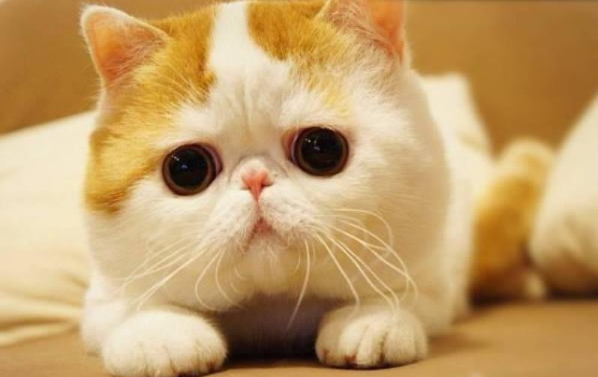
\includegraphics[width=0.5\textwidth]{figures/gatofofo.PNG}
    \caption{Cute cat.}
    \label{fig_gatofofo}
    \caption*{Source: \cite{Babington1993book}}
\end{figure}


You also use subfigures to take your document more organized. The Figure \ref{fig_subfigname} illustrates an example. To cite one specific \index{subfigure} sub-figure you can do this either this \ref{subfig_cutecat} or \ref{subfig_cutestdog}.

\begin{figure}[!ht]
    \centering
    \caption{Caption superior.}
        \subfloat[Cute cat]{
            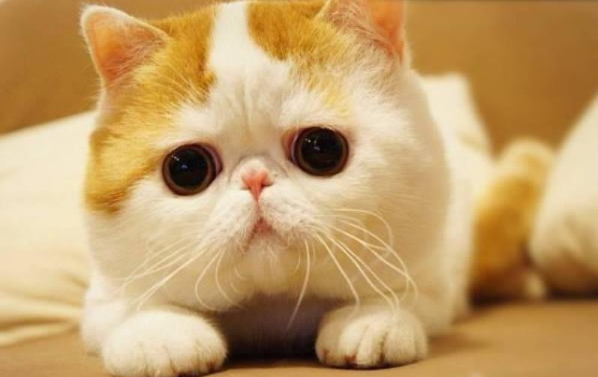
\includegraphics[width=0.3\textwidth]{figures/gatofofo.PNG}
            \label{subfig_cutecat}
        }\qquad
        \subfloat[Custest dog]{
            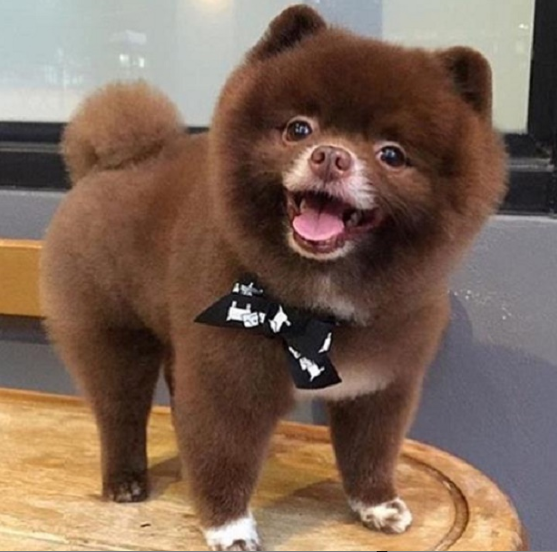
\includegraphics[width=0.3\textwidth]{figures/cachorrofofo.PNG}
            \label{subfig_cutestdog}
        }
    \label{fig_subfigname}
\end{figure}


See \texttt{CTAN: Package subfigure}\footnote{https://ctan.org/pkg/subfigure} for more information. It is possible, yet, to include figures using the package \texttt{subfig}, see e.g. \url{https://tex.stackexchange.com/questions/37581/latex-figures-side-by-side}.

%-----------------------------------
\section{Inserting Outputs Commands and Codes}
\index{output commands}

Excerpts from configuration files and application code may be inserted as figure, as shown in \ref{fig_exemplocomando}. 

To commands and configuration files, it is recommended to use the package \texttt{fancyvrb}. Now, to insert code, you should use the package \texttt{listings} which presents a better presentation of its. In addiction, these both packages allow you insert text/code in external files, without incluse directly in the \LaTeX file.

\begin{figure}[!htb]
\centering
\caption{Inserting Command} 
\begin{Verbatim}[fontsize=\small]
$ dir thesis*
-rw-r--r--  1 joukim users   3650 Set 12 17:56 dissertation.aux
-rw-r--r--  1 joukim users   6366 Set 12 17:43 dissertation.bbl
-rw-r--r--  1 joukim users    290 Set 12 17:56 dissertation.lof
-rw-r--r--  1 joukim users  27937 Set 12 17:56 dissertation.log
-rw-r--r--  1 joukim users    194 Set 12 17:56 dissertation.lot
-rw-r--r--  1 joukim users    715 Set 12 17:56 dissertation.out
-rw-r--r--  1 joukim users 159243 Set 12 17:56 dissertation.pdf
-rw-r--r--  1 joukim users   4559 Set 12 17:47 dissertation.tex
-rw-r--r--  1 joukim users    964 Set 12 17:56 dissertation.toc
\end{Verbatim} 
%$ - esse comentário é para não confundir editor de texto
{\small Source: Blah blah blah, 2018} 
\label{fig_exemplocomando} 
\end{figure}

%-----------------------------------
\section{Tables}
\label{sec_tabelas}

The subsections \ref{subsec_tabsimples} and \ref{subsec_longtable} present examples of \index{table} short table (Table \ref{tab_shorttable}) and long table (Table \ref{tab_longtable}).

%-----------------------------------
\subsection{Example of a Short Table}
\label{subsec_tabsimples}
\index{short table}

We follow the simple rule: horizontal lines only to emphasize the title and in the last line and without vertical lines, as illustrated in Table \ref{tab_shorttable} and Table \ref{tab_longtable} (in Appendix, \ref{appendix}).

To create the tables, we strongly suggest the use of website \texttt{tablegenerator}, available in \url{https://www.tablesgenerator.com/}. It will save your life.

More tips: text should be aligned to the left and keep the numbers with the same number of decimal places and aligned to the right.

\begin{table}[htb]
    \centering
    \caption{Example of a Short Table}
    \label{tab_shorttable}
    \begin{tabular}{lrrr}
    \hline
        Description          & \multicolumn{1}{c}{Value 1} & \multicolumn{1}{c}{Value 2} & \multicolumn{1}{c}{Value 3} \\ \hline
        Cachaça              & 1352,70                     & 1,22                        & 1358,00                     \\
        Caipirinha           & 2005,00                     & 75,21                       & 6873,11                     \\
        Jeropinga            & 8648,00                     & 5,45                        & 852,00                      \\
        Bluepinga            & 4587,55                     & 153,00                      & 53468,00                    \\
        Pagar com Mastercard & 0,00                        & 0,00                        & 0,00                        \\ \hline
    \end{tabular}
\end{table}

%-----------------------------------
\subsection{Example of a Long Table}
\label{subsec_longtable}
\index{long table}

This  long table is in landscape view for better visualization of the information contained. For organization reasons it was sent to the appendix, Section \ref{apendiceA}.


%-----------------------------------
\section{Algorithms}

This section gives an example of Euclid’s \index{algorithm} algorithm shown in \ref{alg_euclid}.

\begin{algorithm}
\caption{My algorithm}\label{alg_euclid}
    \begin{algorithmic}[1]
    \Procedure{MyProcedure}{}
    \State $\textit{stringlen} \gets \text{length of }\textit{string}$
    \State $i \gets \textit{patlen}$
    \BState \emph{top}:
    \If {$i > \textit{stringlen}$} \Return false
    \EndIf
    \State $j \gets \textit{patlen}$
    \BState \emph{loop}:
    \If {$\textit{string}(i) = \textit{path}(j)$}
    \State $j \gets j-1$.
    \State $i \gets i-1$.
    \State \textbf{goto} \emph{loop}.
    \State \textbf{close};
    \EndIf
    \State $i \gets i+\max(\textit{delta}_1(\textit{string}(i)),\textit{delta}_2(j))$.
    \State \textbf{goto} \emph{top}.
    \EndProcedure
    \end{algorithmic}
\end{algorithm}

%-----------------------------------
\section{Some additional links}

In addition, additional links are given bellow:

\begin{itemize}
    \item The \texttt{tocbibind}
package\footnote{http://linorg.usp.br/CTAN/macros/latex/contrib/tocbibind/tocbibind.pdf} - in English.
    \item The \texttt{tocloft}
package\footnote{http://linorg.usp.br/CTAN/macros/latex/contrib/tocloft/tocloft.pdf} - in English.
    \item The \texttt{abntex2cite} package\footnote{http://linorg.usp.br/CTAN/macros/latex/contrib/abntex2/doc/abntex2cite.pdf} - in Portuguese.

\end{itemize}
\chapter[Methodology]{Methodology} 
\label{chp3_methodology} 

\lipsum[2-3]
\chapter[Results]{Results} 
\label{chp4_results} 

\lipsum[2-3]
\chapter[Conclusion]{Conclusion} 
\label{chp5_conclusion} 

\lipsum[2-3]



%-----------------------------------
% Finaliza a parte no bookmark do PDF
% para que se inicie o bookmark na raiz
% e adiciona espaço de parte no Sumário

\phantompart

%-----------------------------------
% Bibliography
\bibliography{references.bib}
\bibliographystyle{abbrvnat}
%\bibliographystyle{unsrtnat}

%-----------------------------------
% POST-TEXTUAL ELEMENTS
%-----------------------------------
\postextual

% Attachments
\begin{anexosenv}
\label{attachments}

%-----------------------------------
\chapter{Looney Tunes} \label{anexoA}

\begin{figure}[htb] 
    \centering
    
\includegraphics[]{figures/looneytunes.jpg}
    \caption{That's all Folks}
    \label{fig_looneytunes}
    \caption*{Fonte: Warner Bross, 1500}
\end{figure}



\end{anexosenv}

% Appendix
%-----------------------------------
\begin{apendicesenv}
\label{appendix}
%-----------------------------------

%-----------------------------------
\chapter{Large Table} \label{apendiceA}

\small
\begin{center}
    \begin{landscape}
        \begin{longtable}{@{\extracolsep{\fill}}ccccccc@{}}
            \caption{Example of a Large Table} \label{tab_longtable}\\
            \hline
            ID &  & Item 1 & Item 2 & Item 3 & Item 4 & Item 5 \\ \hline 
            \endfirsthead
            \multicolumn{7}{c}%
            {\tablename\ \thetable\ -- \textit{Continue in previous page}} \\
            \hline
            \endhead
            \hline 
            \multicolumn{7}{c}{\textit{Continue in next page}} \\
            \endfoot
            \hline
            \endlastfoot
            1       &  & 49   & 16      & 16      & 16      & 16     \\
            2       &  & 72   & 15      & 15      & 15      & 15     \\
            3       &  & 61   & 14      & 14      & 14      & 14     \\
            4       &  & 54   & 13      & 13      & 13      & 13     \\
            5       &  & 57   & 19      & 19      & 19      & 19     \\
            6       &  & 76   & 18      & 18      & 18      & 18     \\
            7       &  & 73   & 11      & 11      & 65      & 65     \\
            8       &  & 70   & 6       & 6       & 11      & 11     \\
            9       &  & 80   & 41      & 5       & 6       & 55     \\
            10      &  & 55   & 5       & 41      & 55      & 6      \\
            11      &  & 69   & 47      & 47      & 64      & 64     \\
            12      &  & 66   & 65      & 65      & 68      & 68     \\
            13      &  & 59   & 17      & 17      & 5       & 58     \\
            14      &  & 78   & 30      & 30      & 41      & 66     \\
            15      &  & 77   & 12      & 55      & 58      & 5      \\
            16      &  & 60   & 34      & 12      & 47      & 41     \\
            17      &  & 63   & 55      & 34      & 66      & 52     \\
            18      &  & 52   & 64      & 64      & 52      & 75     \\
            19      &  & 65   & 68      & 68      & 75      & 47     \\
            20      &  & 56   & 46      & 46      & 17      & 17     \\
            21      &  & 62   & 43      & 43      & 30      & 49     \\
            22      &  & 53   & 27      & 58      & 49      & 77     \\
            23      &  & 67   & 44      & 66      & 12      & 30     \\
            24      &  & 75   & 58      & 27      & 77      & 51     \\
            25      &  & 71   & 40      & 44      & 34      & 72     \\
            26      &  & 51   & 36      & 40      & 51      & 34     \\
            27      &  & 50   & 66      & 52      & 72      & 12     \\
            28      &  & 58   & 52      & 36      & 80      & 80     \\
            29      &  & 79   & 2       & 75      & 63      & 63     \\
            30      &  & 68   & 75      & 2       & 46      & 78     \\
            \hline
        \end{longtable}
    \end{landscape}
\end{center}
\normalsize



\end{apendicesenv}

% Remissive Index
%\renewcommand{\indexname}{Índice Remissivo}
\renewcommand{\indexname}{Index}
\printindex

\end{document}
